
%% bare_conf.tex
%% V1.4
%% 2012/12/27
%% by Michael Shell
%% See:
%% http://www.michaelshell.org/
%% for current contact information.
%%
%% This is a skeleton file demonstrating the use of IEEEtran.cls
%% (requires IEEEtran.cls version 1.8 or later) with an IEEE conference paper.
%%
\documentclass{IEEEtran}
\usepackage[spanish]{babel}
\usepackage[utf8]{inputenc}
\usepackage{enumerate}
\usepackage{cite}
\usepackage{graphicx}  
\usepackage{subfig}

\graphicspath{ {./images/} }

% correct bad hyphenation here
\hyphenation{op-tical net-works semi-conduc-tor}


\usepackage{graphicx}
\begin{document}
%
% paper title
% can use linebreaks \\ within to get better formatting as desired
% Do not put math or special symbols in the title.
\title{Computación paralela y distribuida\\Práctica 1}


% author names and affiliations
% use a multiple column layout for up to three different
% affiliations
\author{\IEEEauthorblockN{Angel Rendón, Andrés Forero\\}
\IEEEauthorblockA{Universidad Nacional Bogotá, Colombia \\
Email:amrendonsa@unal.edu.co, afforeroc@unal.edu.co\\}
}


% make the title area
\maketitle

% As a general rule, do not put math, special symbols or citations
% in the abstract
\begin{abstract}
The abstract goes here. 
\end{abstract}

% no keywords




% For peer review papers, you can put extra information on the cover
% page as needed:
% \ifCLASSOPTIONpeerreview
% \begin{center} \bfseries EDICS Category: 3-BBND \end{center}
% \fi
%
% For peerreview papers, this IEEEtran command inserts a page break and
% creates the second title. It will be ignored for other modes.
\IEEEpeerreviewmaketitle



\section{Introducción.}
% no \IEEEPARstart
This demo file is intended to serve as a ``starter file''
for IEEE conference papers produced under \LaTeX\ using
IEEEtran.cls version 1.8 and later.
% You must have at least 2 lines in the paragraph with the drop letter
% (should never be an issue)
I wish you the best of success.

\hfill mds
 
\hfill December 27, 2012

\subsection{Cálculo de pi.}
Subsection text here.


\subsubsection{Métodos.}
Subsubsection text here.


\begin{figure}[!t]
\centering

\includegraphics[width=\linewidth]{escudo.png}
\caption{Escudo de la Universidad.}
\label{fig_sim}
\end{figure}



\section{Paralelización del algoritmo.}
Aquí va cómo se paralelizó el programa. Siempre es mejor explicar con ayuda de gráficas.



\section{Experimentos y resultados.}
Cómo se probaron los programas. Gráficas, tablas, comentarios.

\begin{figure}[htp]
\centering
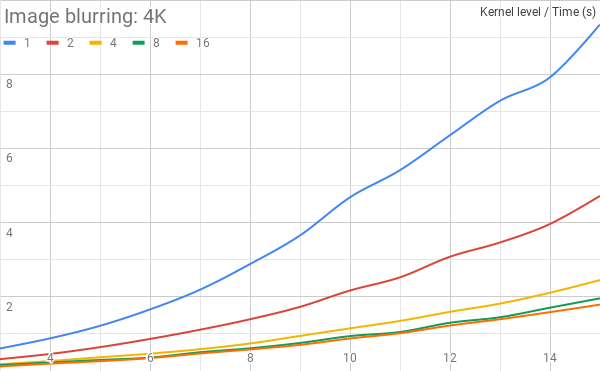
\includegraphics[width=\linewidth]{images/4k.png}
\caption{Resultados para imagen 4K}
\label{4kplot}
\end{figure}

\begin{figure}[htp]
\centering
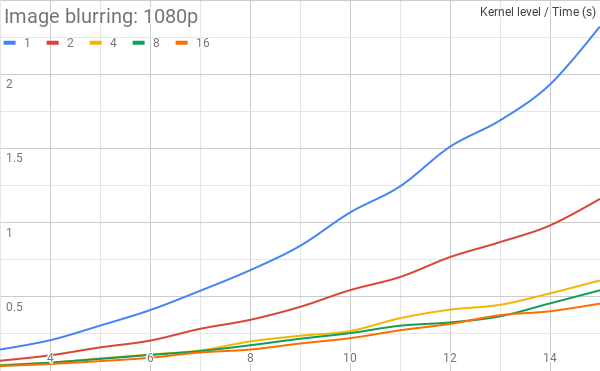
\includegraphics[width=\linewidth]{images/1080p.png}
\caption{Resultados para imagen 1080p}
\label{1080pplot}
\end{figure}

\begin{figure}[htp]
\centering
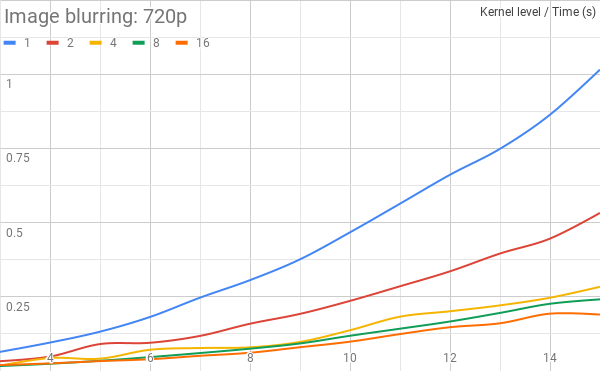
\includegraphics[width=\linewidth]{images/720p.png}
\caption{Resultados para imagen 720p}
\label{720pplot}
\end{figure}


\section*{Conclusiones.}


Conclusiones.

\noindent 
\bibliographystyle{unsrt}       % APS-like style for physics

\bibliography{PARALELOS.bib}
Aquí van las referencias. Ver vídeos para usar con ayuda de Mendeley.



% that's all folks
\end{document}


